The identified issues have been communicated to Reply, along with examples of incorrect values.

At the time of writing, Reply has only fixed issues related to Value tests, meaning that the overall data quality is still going to improve with time.

\begin{figure}
    \centering
    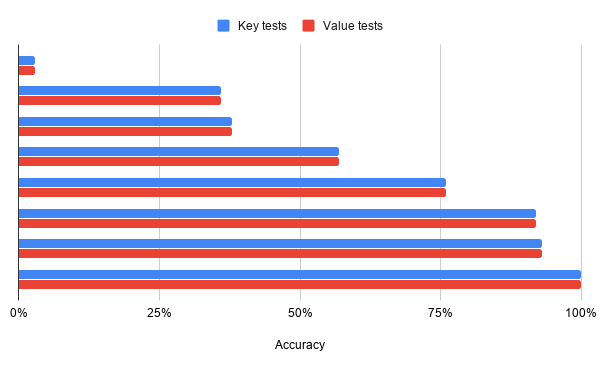
\includegraphics[width=\textwidth]{res/tests/data_val_2.png}
    \caption{Key-Value tests after Reply fixes.}
    \label{fig:tests:data:results_3}
\end{figure}

The tests have been executed once more, obtaining excellent results, as shown in Figure \ref{fig:tests:data:results_3}.

We can see that each Value test has the same accuracy level as their respective Key test.
Value tests, on the other hand are still incomplete.

From these results, we can understand that the ETL process is not yet able to download all the required data, but each downloaded information is correct.
